\documentclass{standalone}
\usepackage{tikz}
\usepackage{amsmath}
\usepackage{xcolor}
\usetikzlibrary{arrows.meta, decorations.pathreplacing, backgrounds, positioning, calc}
% Define custom colors
\definecolor{softyellow}{HTML}{F2D648}
\definecolor{dustyblue}{HTML}{9EB9D4}
\definecolor{berkeleyblue}{RGB}{0, 50, 98}
\definecolor{berkeleygold}{RGB}{253, 181, 21}

\begin{document}

    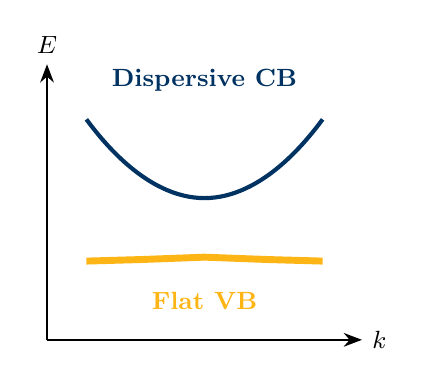
\begin{tikzpicture}[scale=1, 
        >=Stealth,
        every node/.style={font=\small}]
        
        % Axes only
        \draw[->, thick] (-2,-0.5) -- (2,-0.5) node[right] {\textcolor{black}{$k$}};
        \draw[->, thick] (-2,-0.5) -- (-2,3) node[above] {\textcolor{black}{$E$}};
        
        % Dispersive band
        \draw[thick, berkeleyblue, line width=1.5pt] 
          (-1.5,2.3) parabola bend (0,1.3) (1.5,2.3);
              \node[berkeleyblue] at (0,2.8) {\textbf{Dispersive CB}};
      
        % Flat band (with slight curvature)
        \draw[thick, berkeleygold, line width=2.5pt] 
          (-1.5,0.5) -- (-0.8,0.52) -- (0,0.55) -- (0.8,0.52) -- (1.5,0.5);
                  \node[berkeleygold] at (0,0) {\textbf{Flat VB}};
    
    \end{tikzpicture}

\end{document}
